\documentclass[twoside]{book}

% Packages required by doxygen
\usepackage{fixltx2e}
\usepackage{calc}
\usepackage{doxygen}
\usepackage[export]{adjustbox} % also loads graphicx
\usepackage{graphicx}
\usepackage[utf8]{inputenc}
\usepackage{makeidx}
\usepackage{multicol}
\usepackage{multirow}
\PassOptionsToPackage{warn}{textcomp}
\usepackage{textcomp}
\usepackage[nointegrals]{wasysym}
\usepackage[table]{xcolor}

% Font selection
\usepackage[T1]{fontenc}
\usepackage[scaled=.90]{helvet}
\usepackage{courier}
\usepackage{amssymb}
\usepackage{sectsty}
\renewcommand{\familydefault}{\sfdefault}
\allsectionsfont{%
  \fontseries{bc}\selectfont%
  \color{darkgray}%
}
\renewcommand{\DoxyLabelFont}{%
  \fontseries{bc}\selectfont%
  \color{darkgray}%
}
\newcommand{\+}{\discretionary{\mbox{\scriptsize$\hookleftarrow$}}{}{}}

% Page & text layout
\usepackage{geometry}
\geometry{%
  a4paper,%
  top=2.5cm,%
  bottom=2.5cm,%
  left=2.5cm,%
  right=2.5cm%
}
\tolerance=750
\hfuzz=15pt
\hbadness=750
\setlength{\emergencystretch}{15pt}
\setlength{\parindent}{0cm}
\setlength{\parskip}{3ex plus 2ex minus 2ex}
\makeatletter
\renewcommand{\paragraph}{%
  \@startsection{paragraph}{4}{0ex}{-1.0ex}{1.0ex}{%
    \normalfont\normalsize\bfseries\SS@parafont%
  }%
}
\renewcommand{\subparagraph}{%
  \@startsection{subparagraph}{5}{0ex}{-1.0ex}{1.0ex}{%
    \normalfont\normalsize\bfseries\SS@subparafont%
  }%
}
\makeatother

% Headers & footers
\usepackage{fancyhdr}
\pagestyle{fancyplain}
\fancyhead[LE]{\fancyplain{}{\bfseries\thepage}}
\fancyhead[CE]{\fancyplain{}{}}
\fancyhead[RE]{\fancyplain{}{\bfseries\leftmark}}
\fancyhead[LO]{\fancyplain{}{\bfseries\rightmark}}
\fancyhead[CO]{\fancyplain{}{}}
\fancyhead[RO]{\fancyplain{}{\bfseries\thepage}}
\fancyfoot[LE]{\fancyplain{}{}}
\fancyfoot[CE]{\fancyplain{}{}}
\fancyfoot[RE]{\fancyplain{}{\bfseries\scriptsize Generated by Doxygen }}
\fancyfoot[LO]{\fancyplain{}{\bfseries\scriptsize Generated by Doxygen }}
\fancyfoot[CO]{\fancyplain{}{}}
\fancyfoot[RO]{\fancyplain{}{}}
\renewcommand{\footrulewidth}{0.4pt}
\renewcommand{\chaptermark}[1]{%
  \markboth{#1}{}%
}
\renewcommand{\sectionmark}[1]{%
  \markright{\thesection\ #1}%
}

% Indices & bibliography
\usepackage{natbib}
\usepackage[titles]{tocloft}
\setcounter{tocdepth}{3}
\setcounter{secnumdepth}{5}
\makeindex

% Hyperlinks (required, but should be loaded last)
\usepackage{ifpdf}
\ifpdf
  \usepackage[pdftex,pagebackref=true]{hyperref}
\else
  \usepackage[ps2pdf,pagebackref=true]{hyperref}
\fi
\hypersetup{%
  colorlinks=true,%
  linkcolor=blue,%
  citecolor=blue,%
  unicode%
}

% Custom commands
\newcommand{\clearemptydoublepage}{%
  \newpage{\pagestyle{empty}\cleardoublepage}%
}

\usepackage{caption}
\captionsetup{labelsep=space,justification=centering,font={bf},singlelinecheck=off,skip=4pt,position=top}

%===== C O N T E N T S =====

\begin{document}

% Titlepage & ToC
\hypersetup{pageanchor=false,
             bookmarksnumbered=true,
             pdfencoding=unicode
            }
\pagenumbering{alph}
\begin{titlepage}
\vspace*{7cm}
\begin{center}%
{\Large My Project }\\
\vspace*{1cm}
{\large Generated by Doxygen 1.8.13}\\
\end{center}
\end{titlepage}
\clearemptydoublepage
\pagenumbering{roman}
\tableofcontents
\clearemptydoublepage
\pagenumbering{arabic}
\hypersetup{pageanchor=true}

%--- Begin generated contents ---
\chapter{Second\+\_\+assignment}
\label{md__r_e_a_d_m_e}
\Hypertarget{md__r_e_a_d_m_e}
\subsection*{Introduction}

In this repository it\textquotesingle{}s implemented a simple user interface to permit to a generic robot to move in a definite map by avoiding the obstacles. In particular with this interface, user can ask to the robot to move in a random position between the six positions that are allowed, to move in a user defined position, to follow the external walls of the map and to stop in the last robot position.

To be executed this interface needs other three packages (slam\+\_\+gmapping, final\+\_\+assignment and robot\+\_\+description), without which is not possible to run this code, since some services that are required are contained in these packages.

Note\+: this code was developed for R\+OS melodic, but can be executed also in other R\+OS distributions by downloading the indicated slam\+\_\+gmapping, final\+\_\+assignment and robot\+\_\+description packages for the considered distribution.

In this repository there are four folders\+:


\begin{DoxyItemize}
\item launch
\item scripts
\item src
\item srv
\end{DoxyItemize}

The first one contains a launch file that permits to execute the entire program, so by launching the my\+\_\+robot\+\_\+controller.\+launch it\textquotesingle{}s possible to run the robot user interface and other nodes, like move\+\_\+base and wall\+\_\+follower, that are already implemented and permit the robot to move in a certain position and to follow the external walls.

In the \char`\"{}scripts\char`\"{} folder it\textquotesingle{}s contained the \hyperlink{robot__user__interface_8py}{robot\+\_\+user\+\_\+interface.\+py} script, that is the user interface of the program. Here the program asks the user to give him the commands to decide wich operation should it execute and to do that it calls the services that are launched previously with the launch file.

The \char`\"{}src\char`\"{} folder contains the \hyperlink{_server__second__assignment_8cpp}{server\+\_\+second\+\_\+assignment.\+cpp} code, that is a server that returns randomly one of the six allowed positions.

The \char`\"{}srv\char`\"{} folder contains a file to define the type of the data that are returned from the server.

\subsection*{Comunication between nodes}



~\newline


As it\textquotesingle{}s possible to see in the picture, this is how the nodes communicate to each others\+: what it\textquotesingle{}s interesting to consider is that the \hyperlink{namespacerobot__user__interface}{robot\+\_\+user\+\_\+interface} node gets the odom data to obtain the position of the robot in the map (by subscribing to the odom service) and can set the velocity of the robot by publishing a cmd\+\_\+vel message to the Twist publisher. The \hyperlink{namespacerobot__user__interface}{robot\+\_\+user\+\_\+interface} also moves the robot in a certain position by sending a message of type move\+\_\+base\+\_\+msgs/\+Move\+Base\+Action\+Goal.

\subsection*{Robot behaviors and software architecture}

\subsubsection*{Software architecture}

First, at the beginning of the execution the nodes /robot\+\_\+user\+\_\+interface and /server\+\_\+second\+\_\+assignment initialize the publishers and the subscribers with respect to the other running nodes. After that the main part of the \hyperlink{namespacerobot__user__interface}{robot\+\_\+user\+\_\+interface} has to ask in an infinite loop the commands to the user

1) To randomly move in one of the allowed positions 2) Ask user to choose the target position for the robot 3) Let the robot following the external walls 4) Stop the robot

As previously mentioned, not all the positons are allowed, the only target position that robot is allowed to reach are \mbox{[}-\/4, -\/3\mbox{]}, \mbox{[}5, -\/3\mbox{]}, \mbox{[}-\/4, 2\mbox{]}, \mbox{[}-\/4, 7\mbox{]}, \mbox{[}5, -\/7\mbox{]}, \mbox{[}5, 1\mbox{]}, so if user chooses another position the program asks him to digit it agin.

When the position is randomly chosen the \hyperlink{namespacerobot__user__interface}{robot\+\_\+user\+\_\+interface} node sends a request to server\+\_\+second\+\_\+assignment node, which will return one of the allowed positions. To do that the server generate a random number from 0 to 5 that is utilized as the index of the array in wich are contained the allowed positions. After having received the position either from the server or from the user, to move the robot it\textquotesingle{}s set a field goal with the x and y coordinates of the target to reach

To let the robot follow the external walls, the program only has to call the wall\+\_\+follower service while to stop the robot the linear velocity is set to 0 and to make sure that the robot won\textquotesingle{}t go to another position user asks him before, the program sets a field goal with the coordinates of the position of the robot when it was ordered him to stop.

\subsubsection*{Behaviors}

As it\textquotesingle{}s possible to notice by having a look to the R\+V\+IZ simulation, at the beginning the robot doesn\textquotesingle{}t completely know the entire map, so to move in a certain position it will learn the map by scanning it while it is moving. This means that sometimes when the robot has to reach a position it doesn\textquotesingle{}t know, it goes in a wrong direction at the beginning and when robot understands it, it comes back and searches for another path to follow. At the end, when the robot has seen the entire map, it doesn\textquotesingle{}t fail the optimal path to reach a certain position anymore.

\subsection*{Considerations}

The robot can successfully reach the positions and in general move avoiding the obstacles. The algorithm that is implemented to understand the map in which it moves is optimal in this case, since the dimension of the entire map is limited, maybe in a bigger and more complicate map it\textquotesingle{}s possible that robot can get lost more time before it can learn the entire map.

In the code to move in a certain position is adopted the move\+\_\+base algorithm, it could also be possible to do it by implementing the bug0 algorithm and even ask to user to decide which kind of algorithm robot should use.

\subsection*{How to run the code}

To run the code it\textquotesingle{}s necessary to have the slam\+\_\+gmapping, final\+\_\+assignment and robot\+\_\+description packages inside its own workspace, then clone also this repository inside it and then, after having gone in your workspace folder in the terminal, execute the following commands\+:


\begin{DoxyItemize}
\item roscore \&
\item catkin\+\_\+make
\item roslaunch final\+\_\+assignment simulation\+\_\+gmapping.\+launch
\item roslaunch second\+\_\+assignment my\+\_\+robot\+\_\+controller.\+launch
\end{DoxyItemize}

Then you should see the R\+V\+IZ and Gazeebo simulation of the robot and of the map, then by digiting the commands on the terminal and by following the instructions on the user interface you can send commands to the robot. 
\chapter{Namespace Index}
\section{Namespace List}
Here is a list of all namespaces with brief descriptions\+:\begin{DoxyCompactList}
\item\contentsline{section}{\hyperlink{namespacerobot__user__interface}{robot\+\_\+user\+\_\+interface} }{\pageref{namespacerobot__user__interface}}{}
\end{DoxyCompactList}

\chapter{File Index}
\section{File List}
Here is a list of all files with brief descriptions\+:\begin{DoxyCompactList}
\item\contentsline{section}{scripts/\hyperlink{robot__user__interface_8py}{robot\+\_\+user\+\_\+interface.\+py} }{\pageref{robot__user__interface_8py}}{}
\item\contentsline{section}{src/\hyperlink{_server__second__assignment_8cpp}{Server\+\_\+second\+\_\+assignment.\+cpp} }{\pageref{_server__second__assignment_8cpp}}{}
\end{DoxyCompactList}

\chapter{Namespace Documentation}
\hypertarget{namespacerobot__user__interface}{}\section{robot\+\_\+user\+\_\+interface Namespace Reference}
\label{namespacerobot__user__interface}\index{robot\+\_\+user\+\_\+interface@{robot\+\_\+user\+\_\+interface}}
\subsection*{Functions}
\begin{DoxyCompactItemize}
\item 
def \hyperlink{namespacerobot__user__interface_ac0334cd2b07f8bc4474062eaaceab902}{position\+Callback} (msg)
\begin{DoxyCompactList}\small\item\em Callback to constantly get the robot position. \end{DoxyCompactList}\item 
def \hyperlink{namespacerobot__user__interface_af8347c189738ddfec5e6582d1a8839fa}{user\+\_\+set\+\_\+position} ()
\begin{DoxyCompactList}\small\item\em Function to get a new position from the user and check that it\textquotesingle{}s one of the catchable positions. \end{DoxyCompactList}\item 
def \hyperlink{namespacerobot__user__interface_a137d7201aae4fbac4990876227d162f1}{move\+\_\+randomly} ()
\begin{DoxyCompactList}\small\item\em Function to move in the direction received from the server. \end{DoxyCompactList}\item 
def \hyperlink{namespacerobot__user__interface_a74312af906c16599bef2c4ade3ef87a4}{follow\+\_\+wall} ()
\begin{DoxyCompactList}\small\item\em Function to make the robot follow the external walls. \end{DoxyCompactList}\item 
def \hyperlink{namespacerobot__user__interface_a70a457867820599c4b2a30f4027dd513}{stop\+\_\+robot} ()
\begin{DoxyCompactList}\small\item\em To stop the robot the linear velocity values are set to 0, evenmore the target to reach is set to the position in wich robot is, so that to make sure it won\textquotesingle{}t try to reach another position. \end{DoxyCompactList}\item 
def \hyperlink{namespacerobot__user__interface_ac0177573471df46aa7986edba5620184}{set\+\_\+target\+\_\+position} (target\+\_\+x, target\+\_\+y)
\begin{DoxyCompactList}\small\item\em This function get two parameters, target\+\_\+x and target\+\_\+y and set the target position in wich robot has to go. \end{DoxyCompactList}\item 
def \hyperlink{namespacerobot__user__interface_a20558ce4717c6399da8e04e96858203f}{distance} ()
\begin{DoxyCompactList}\small\item\em Function to estimate the value of the distance between the robot positon and the target it has to reach. \end{DoxyCompactList}\item 
def \hyperlink{namespacerobot__user__interface_a6c919b4750dd38ddd929c5e456053de0}{main} ()
\end{DoxyCompactItemize}
\subsection*{Variables}
\begin{DoxyCompactItemize}
\item 
\hyperlink{namespacerobot__user__interface_a93557af62ae5a9f9fb406de12d599a58}{actual\+\_\+position} = Point()
\item 
int \hyperlink{namespacerobot__user__interface_aa49c4c4b4c031611deca926a34deb345}{goal\+\_\+x} = 0
\begin{DoxyCompactList}\small\item\em Variables to save the value of the target robot has to reach. \end{DoxyCompactList}\item 
int \hyperlink{namespacerobot__user__interface_aee93dc3e48f178d62b1209aa13232be2}{goal\+\_\+y} = 0
\item 
bool \hyperlink{namespacerobot__user__interface_ab96d4afbc6f7d4bb5019beec53e4615d}{notify} = False
\begin{DoxyCompactList}\small\item\em Variable to generate a message of reached position in the position\+Callback. \end{DoxyCompactList}\item 
bool \hyperlink{namespacerobot__user__interface_ab735683088fe7d67ce16d40c53b3208c}{set\+\_\+target} = False
\item 
int \hyperlink{namespacerobot__user__interface_a57ca0e32cc10313871da599206689de6}{dist} = 0
\begin{DoxyCompactList}\small\item\em Initialize the distance to the target. \end{DoxyCompactList}\item 
\hyperlink{namespacerobot__user__interface_ad8e7e9dc5f614912b17e97229d3bc726}{pub\+\_\+move\+\_\+base} = None
\begin{DoxyCompactList}\small\item\em Initialize the publishers. \end{DoxyCompactList}\item 
\hyperlink{namespacerobot__user__interface_aa95d3e42b12dbcb906f08ec10450e436}{pub\+\_\+twist} = None
\item 
\hyperlink{namespacerobot__user__interface_a18cc77d7f27b808397c9d58367a25280}{sub\+\_\+odom} = None
\begin{DoxyCompactList}\small\item\em Initialize the odom subscriber. \end{DoxyCompactList}\item 
\hyperlink{namespacerobot__user__interface_a95d6798bc3ba3f2e590443ca7ad8d7d4}{srv\+\_\+client\+\_\+wall\+\_\+follower} = None
\begin{DoxyCompactList}\small\item\em Initialize the wall\+\_\+follower client. \end{DoxyCompactList}\end{DoxyCompactItemize}


\subsection{Function Documentation}
\mbox{\Hypertarget{namespacerobot__user__interface_a20558ce4717c6399da8e04e96858203f}\label{namespacerobot__user__interface_a20558ce4717c6399da8e04e96858203f}} 
\index{robot\+\_\+user\+\_\+interface@{robot\+\_\+user\+\_\+interface}!distance@{distance}}
\index{distance@{distance}!robot\+\_\+user\+\_\+interface@{robot\+\_\+user\+\_\+interface}}
\subsubsection{\texorpdfstring{distance()}{distance()}}
{\footnotesize\ttfamily def robot\+\_\+user\+\_\+interface.\+distance (\begin{DoxyParamCaption}{ }\end{DoxyParamCaption})}



Function to estimate the value of the distance between the robot positon and the target it has to reach. 



Definition at line 212 of file robot\+\_\+user\+\_\+interface.\+py.

\mbox{\Hypertarget{namespacerobot__user__interface_a74312af906c16599bef2c4ade3ef87a4}\label{namespacerobot__user__interface_a74312af906c16599bef2c4ade3ef87a4}} 
\index{robot\+\_\+user\+\_\+interface@{robot\+\_\+user\+\_\+interface}!follow\+\_\+wall@{follow\+\_\+wall}}
\index{follow\+\_\+wall@{follow\+\_\+wall}!robot\+\_\+user\+\_\+interface@{robot\+\_\+user\+\_\+interface}}
\subsubsection{\texorpdfstring{follow\+\_\+wall()}{follow\_wall()}}
{\footnotesize\ttfamily def robot\+\_\+user\+\_\+interface.\+follow\+\_\+wall (\begin{DoxyParamCaption}{ }\end{DoxyParamCaption})}



Function to make the robot follow the external walls. 



Definition at line 130 of file robot\+\_\+user\+\_\+interface.\+py.

\mbox{\Hypertarget{namespacerobot__user__interface_a6c919b4750dd38ddd929c5e456053de0}\label{namespacerobot__user__interface_a6c919b4750dd38ddd929c5e456053de0}} 
\index{robot\+\_\+user\+\_\+interface@{robot\+\_\+user\+\_\+interface}!main@{main}}
\index{main@{main}!robot\+\_\+user\+\_\+interface@{robot\+\_\+user\+\_\+interface}}
\subsubsection{\texorpdfstring{main()}{main()}}
{\footnotesize\ttfamily def robot\+\_\+user\+\_\+interface.\+main (\begin{DoxyParamCaption}{ }\end{DoxyParamCaption})}



Definition at line 227 of file robot\+\_\+user\+\_\+interface.\+py.

\mbox{\Hypertarget{namespacerobot__user__interface_a137d7201aae4fbac4990876227d162f1}\label{namespacerobot__user__interface_a137d7201aae4fbac4990876227d162f1}} 
\index{robot\+\_\+user\+\_\+interface@{robot\+\_\+user\+\_\+interface}!move\+\_\+randomly@{move\+\_\+randomly}}
\index{move\+\_\+randomly@{move\+\_\+randomly}!robot\+\_\+user\+\_\+interface@{robot\+\_\+user\+\_\+interface}}
\subsubsection{\texorpdfstring{move\+\_\+randomly()}{move\_randomly()}}
{\footnotesize\ttfamily def robot\+\_\+user\+\_\+interface.\+move\+\_\+randomly (\begin{DoxyParamCaption}{ }\end{DoxyParamCaption})}



Function to move in the direction received from the server. 



Definition at line 113 of file robot\+\_\+user\+\_\+interface.\+py.

\mbox{\Hypertarget{namespacerobot__user__interface_ac0334cd2b07f8bc4474062eaaceab902}\label{namespacerobot__user__interface_ac0334cd2b07f8bc4474062eaaceab902}} 
\index{robot\+\_\+user\+\_\+interface@{robot\+\_\+user\+\_\+interface}!position\+Callback@{position\+Callback}}
\index{position\+Callback@{position\+Callback}!robot\+\_\+user\+\_\+interface@{robot\+\_\+user\+\_\+interface}}
\subsubsection{\texorpdfstring{position\+Callback()}{positionCallback()}}
{\footnotesize\ttfamily def robot\+\_\+user\+\_\+interface.\+position\+Callback (\begin{DoxyParamCaption}\item[{}]{msg }\end{DoxyParamCaption})}



Callback to constantly get the robot position. 



Definition at line 42 of file robot\+\_\+user\+\_\+interface.\+py.

\mbox{\Hypertarget{namespacerobot__user__interface_ac0177573471df46aa7986edba5620184}\label{namespacerobot__user__interface_ac0177573471df46aa7986edba5620184}} 
\index{robot\+\_\+user\+\_\+interface@{robot\+\_\+user\+\_\+interface}!set\+\_\+target\+\_\+position@{set\+\_\+target\+\_\+position}}
\index{set\+\_\+target\+\_\+position@{set\+\_\+target\+\_\+position}!robot\+\_\+user\+\_\+interface@{robot\+\_\+user\+\_\+interface}}
\subsubsection{\texorpdfstring{set\+\_\+target\+\_\+position()}{set\_target\_position()}}
{\footnotesize\ttfamily def robot\+\_\+user\+\_\+interface.\+set\+\_\+target\+\_\+position (\begin{DoxyParamCaption}\item[{}]{target\+\_\+x,  }\item[{}]{target\+\_\+y }\end{DoxyParamCaption})}



This function get two parameters, target\+\_\+x and target\+\_\+y and set the target position in wich robot has to go. 



Definition at line 180 of file robot\+\_\+user\+\_\+interface.\+py.

\mbox{\Hypertarget{namespacerobot__user__interface_a70a457867820599c4b2a30f4027dd513}\label{namespacerobot__user__interface_a70a457867820599c4b2a30f4027dd513}} 
\index{robot\+\_\+user\+\_\+interface@{robot\+\_\+user\+\_\+interface}!stop\+\_\+robot@{stop\+\_\+robot}}
\index{stop\+\_\+robot@{stop\+\_\+robot}!robot\+\_\+user\+\_\+interface@{robot\+\_\+user\+\_\+interface}}
\subsubsection{\texorpdfstring{stop\+\_\+robot()}{stop\_robot()}}
{\footnotesize\ttfamily def robot\+\_\+user\+\_\+interface.\+stop\+\_\+robot (\begin{DoxyParamCaption}{ }\end{DoxyParamCaption})}



To stop the robot the linear velocity values are set to 0, evenmore the target to reach is set to the position in wich robot is, so that to make sure it won\textquotesingle{}t try to reach another position. 



Definition at line 141 of file robot\+\_\+user\+\_\+interface.\+py.

\mbox{\Hypertarget{namespacerobot__user__interface_af8347c189738ddfec5e6582d1a8839fa}\label{namespacerobot__user__interface_af8347c189738ddfec5e6582d1a8839fa}} 
\index{robot\+\_\+user\+\_\+interface@{robot\+\_\+user\+\_\+interface}!user\+\_\+set\+\_\+position@{user\+\_\+set\+\_\+position}}
\index{user\+\_\+set\+\_\+position@{user\+\_\+set\+\_\+position}!robot\+\_\+user\+\_\+interface@{robot\+\_\+user\+\_\+interface}}
\subsubsection{\texorpdfstring{user\+\_\+set\+\_\+position()}{user\_set\_position()}}
{\footnotesize\ttfamily def robot\+\_\+user\+\_\+interface.\+user\+\_\+set\+\_\+position (\begin{DoxyParamCaption}{ }\end{DoxyParamCaption})}



Function to get a new position from the user and check that it\textquotesingle{}s one of the catchable positions. 



Definition at line 54 of file robot\+\_\+user\+\_\+interface.\+py.



\subsection{Variable Documentation}
\mbox{\Hypertarget{namespacerobot__user__interface_a93557af62ae5a9f9fb406de12d599a58}\label{namespacerobot__user__interface_a93557af62ae5a9f9fb406de12d599a58}} 
\index{robot\+\_\+user\+\_\+interface@{robot\+\_\+user\+\_\+interface}!actual\+\_\+position@{actual\+\_\+position}}
\index{actual\+\_\+position@{actual\+\_\+position}!robot\+\_\+user\+\_\+interface@{robot\+\_\+user\+\_\+interface}}
\subsubsection{\texorpdfstring{actual\+\_\+position}{actual\_position}}
{\footnotesize\ttfamily robot\+\_\+user\+\_\+interface.\+actual\+\_\+position = Point()}



Definition at line 15 of file robot\+\_\+user\+\_\+interface.\+py.

\mbox{\Hypertarget{namespacerobot__user__interface_a57ca0e32cc10313871da599206689de6}\label{namespacerobot__user__interface_a57ca0e32cc10313871da599206689de6}} 
\index{robot\+\_\+user\+\_\+interface@{robot\+\_\+user\+\_\+interface}!dist@{dist}}
\index{dist@{dist}!robot\+\_\+user\+\_\+interface@{robot\+\_\+user\+\_\+interface}}
\subsubsection{\texorpdfstring{dist}{dist}}
{\footnotesize\ttfamily int robot\+\_\+user\+\_\+interface.\+dist = 0}



Initialize the distance to the target. 



Definition at line 27 of file robot\+\_\+user\+\_\+interface.\+py.

\mbox{\Hypertarget{namespacerobot__user__interface_aa49c4c4b4c031611deca926a34deb345}\label{namespacerobot__user__interface_aa49c4c4b4c031611deca926a34deb345}} 
\index{robot\+\_\+user\+\_\+interface@{robot\+\_\+user\+\_\+interface}!goal\+\_\+x@{goal\+\_\+x}}
\index{goal\+\_\+x@{goal\+\_\+x}!robot\+\_\+user\+\_\+interface@{robot\+\_\+user\+\_\+interface}}
\subsubsection{\texorpdfstring{goal\+\_\+x}{goal\_x}}
{\footnotesize\ttfamily int robot\+\_\+user\+\_\+interface.\+goal\+\_\+x = 0}



Variables to save the value of the target robot has to reach. 



Definition at line 18 of file robot\+\_\+user\+\_\+interface.\+py.

\mbox{\Hypertarget{namespacerobot__user__interface_aee93dc3e48f178d62b1209aa13232be2}\label{namespacerobot__user__interface_aee93dc3e48f178d62b1209aa13232be2}} 
\index{robot\+\_\+user\+\_\+interface@{robot\+\_\+user\+\_\+interface}!goal\+\_\+y@{goal\+\_\+y}}
\index{goal\+\_\+y@{goal\+\_\+y}!robot\+\_\+user\+\_\+interface@{robot\+\_\+user\+\_\+interface}}
\subsubsection{\texorpdfstring{goal\+\_\+y}{goal\_y}}
{\footnotesize\ttfamily int robot\+\_\+user\+\_\+interface.\+goal\+\_\+y = 0}



Definition at line 19 of file robot\+\_\+user\+\_\+interface.\+py.

\mbox{\Hypertarget{namespacerobot__user__interface_ab96d4afbc6f7d4bb5019beec53e4615d}\label{namespacerobot__user__interface_ab96d4afbc6f7d4bb5019beec53e4615d}} 
\index{robot\+\_\+user\+\_\+interface@{robot\+\_\+user\+\_\+interface}!notify@{notify}}
\index{notify@{notify}!robot\+\_\+user\+\_\+interface@{robot\+\_\+user\+\_\+interface}}
\subsubsection{\texorpdfstring{notify}{notify}}
{\footnotesize\ttfamily bool robot\+\_\+user\+\_\+interface.\+notify = False}



Variable to generate a message of reached position in the position\+Callback. 



Definition at line 22 of file robot\+\_\+user\+\_\+interface.\+py.

\mbox{\Hypertarget{namespacerobot__user__interface_ad8e7e9dc5f614912b17e97229d3bc726}\label{namespacerobot__user__interface_ad8e7e9dc5f614912b17e97229d3bc726}} 
\index{robot\+\_\+user\+\_\+interface@{robot\+\_\+user\+\_\+interface}!pub\+\_\+move\+\_\+base@{pub\+\_\+move\+\_\+base}}
\index{pub\+\_\+move\+\_\+base@{pub\+\_\+move\+\_\+base}!robot\+\_\+user\+\_\+interface@{robot\+\_\+user\+\_\+interface}}
\subsubsection{\texorpdfstring{pub\+\_\+move\+\_\+base}{pub\_move\_base}}
{\footnotesize\ttfamily robot\+\_\+user\+\_\+interface.\+pub\+\_\+move\+\_\+base = None}



Initialize the publishers. 



Definition at line 31 of file robot\+\_\+user\+\_\+interface.\+py.

\mbox{\Hypertarget{namespacerobot__user__interface_aa95d3e42b12dbcb906f08ec10450e436}\label{namespacerobot__user__interface_aa95d3e42b12dbcb906f08ec10450e436}} 
\index{robot\+\_\+user\+\_\+interface@{robot\+\_\+user\+\_\+interface}!pub\+\_\+twist@{pub\+\_\+twist}}
\index{pub\+\_\+twist@{pub\+\_\+twist}!robot\+\_\+user\+\_\+interface@{robot\+\_\+user\+\_\+interface}}
\subsubsection{\texorpdfstring{pub\+\_\+twist}{pub\_twist}}
{\footnotesize\ttfamily robot\+\_\+user\+\_\+interface.\+pub\+\_\+twist = None}



Definition at line 32 of file robot\+\_\+user\+\_\+interface.\+py.

\mbox{\Hypertarget{namespacerobot__user__interface_ab735683088fe7d67ce16d40c53b3208c}\label{namespacerobot__user__interface_ab735683088fe7d67ce16d40c53b3208c}} 
\index{robot\+\_\+user\+\_\+interface@{robot\+\_\+user\+\_\+interface}!set\+\_\+target@{set\+\_\+target}}
\index{set\+\_\+target@{set\+\_\+target}!robot\+\_\+user\+\_\+interface@{robot\+\_\+user\+\_\+interface}}
\subsubsection{\texorpdfstring{set\+\_\+target}{set\_target}}
{\footnotesize\ttfamily bool robot\+\_\+user\+\_\+interface.\+set\+\_\+target = False}



Definition at line 24 of file robot\+\_\+user\+\_\+interface.\+py.

\mbox{\Hypertarget{namespacerobot__user__interface_a95d6798bc3ba3f2e590443ca7ad8d7d4}\label{namespacerobot__user__interface_a95d6798bc3ba3f2e590443ca7ad8d7d4}} 
\index{robot\+\_\+user\+\_\+interface@{robot\+\_\+user\+\_\+interface}!srv\+\_\+client\+\_\+wall\+\_\+follower@{srv\+\_\+client\+\_\+wall\+\_\+follower}}
\index{srv\+\_\+client\+\_\+wall\+\_\+follower@{srv\+\_\+client\+\_\+wall\+\_\+follower}!robot\+\_\+user\+\_\+interface@{robot\+\_\+user\+\_\+interface}}
\subsubsection{\texorpdfstring{srv\+\_\+client\+\_\+wall\+\_\+follower}{srv\_client\_wall\_follower}}
{\footnotesize\ttfamily robot\+\_\+user\+\_\+interface.\+srv\+\_\+client\+\_\+wall\+\_\+follower = None}



Initialize the wall\+\_\+follower client. 



Definition at line 38 of file robot\+\_\+user\+\_\+interface.\+py.

\mbox{\Hypertarget{namespacerobot__user__interface_a18cc77d7f27b808397c9d58367a25280}\label{namespacerobot__user__interface_a18cc77d7f27b808397c9d58367a25280}} 
\index{robot\+\_\+user\+\_\+interface@{robot\+\_\+user\+\_\+interface}!sub\+\_\+odom@{sub\+\_\+odom}}
\index{sub\+\_\+odom@{sub\+\_\+odom}!robot\+\_\+user\+\_\+interface@{robot\+\_\+user\+\_\+interface}}
\subsubsection{\texorpdfstring{sub\+\_\+odom}{sub\_odom}}
{\footnotesize\ttfamily robot\+\_\+user\+\_\+interface.\+sub\+\_\+odom = None}



Initialize the odom subscriber. 



Definition at line 35 of file robot\+\_\+user\+\_\+interface.\+py.


\chapter{File Documentation}
\hypertarget{_r_e_a_d_m_e_8md}{}\section{R\+E\+A\+D\+M\+E.\+md File Reference}
\label{_r_e_a_d_m_e_8md}\index{R\+E\+A\+D\+M\+E.\+md@{R\+E\+A\+D\+M\+E.\+md}}

\hypertarget{robot__user__interface_8py}{}\section{scripts/robot\+\_\+user\+\_\+interface.py File Reference}
\label{robot__user__interface_8py}\index{scripts/robot\+\_\+user\+\_\+interface.\+py@{scripts/robot\+\_\+user\+\_\+interface.\+py}}
\subsection*{Namespaces}
\begin{DoxyCompactItemize}
\item 
 \hyperlink{namespacerobot__user__interface}{robot\+\_\+user\+\_\+interface}
\end{DoxyCompactItemize}
\subsection*{Functions}
\begin{DoxyCompactItemize}
\item 
def \hyperlink{namespacerobot__user__interface_ac0334cd2b07f8bc4474062eaaceab902}{robot\+\_\+user\+\_\+interface.\+position\+Callback} (msg)
\begin{DoxyCompactList}\small\item\em Callback to constantly get the robot position. \end{DoxyCompactList}\item 
def \hyperlink{namespacerobot__user__interface_af8347c189738ddfec5e6582d1a8839fa}{robot\+\_\+user\+\_\+interface.\+user\+\_\+set\+\_\+position} ()
\begin{DoxyCompactList}\small\item\em Function to get a new position from the user and check that it\textquotesingle{}s one of the catchable positions. \end{DoxyCompactList}\item 
def \hyperlink{namespacerobot__user__interface_a137d7201aae4fbac4990876227d162f1}{robot\+\_\+user\+\_\+interface.\+move\+\_\+randomly} ()
\begin{DoxyCompactList}\small\item\em Function to move in the direction received from the server. \end{DoxyCompactList}\item 
def \hyperlink{namespacerobot__user__interface_a74312af906c16599bef2c4ade3ef87a4}{robot\+\_\+user\+\_\+interface.\+follow\+\_\+wall} ()
\begin{DoxyCompactList}\small\item\em Function to make the robot follow the external walls. \end{DoxyCompactList}\item 
def \hyperlink{namespacerobot__user__interface_a70a457867820599c4b2a30f4027dd513}{robot\+\_\+user\+\_\+interface.\+stop\+\_\+robot} ()
\begin{DoxyCompactList}\small\item\em To stop the robot the linear velocity values are set to 0, evenmore the target to reach is set to the position in wich robot is, so that to make sure it won\textquotesingle{}t try to reach another position. \end{DoxyCompactList}\item 
def \hyperlink{namespacerobot__user__interface_ac0177573471df46aa7986edba5620184}{robot\+\_\+user\+\_\+interface.\+set\+\_\+target\+\_\+position} (target\+\_\+x, target\+\_\+y)
\begin{DoxyCompactList}\small\item\em This function get two parameters, target\+\_\+x and target\+\_\+y and set the target position in wich robot has to go. \end{DoxyCompactList}\item 
def \hyperlink{namespacerobot__user__interface_a20558ce4717c6399da8e04e96858203f}{robot\+\_\+user\+\_\+interface.\+distance} ()
\begin{DoxyCompactList}\small\item\em Function to estimate the value of the distance between the robot positon and the target it has to reach. \end{DoxyCompactList}\item 
def \hyperlink{namespacerobot__user__interface_a6c919b4750dd38ddd929c5e456053de0}{robot\+\_\+user\+\_\+interface.\+main} ()
\end{DoxyCompactItemize}
\subsection*{Variables}
\begin{DoxyCompactItemize}
\item 
\hyperlink{namespacerobot__user__interface_a93557af62ae5a9f9fb406de12d599a58}{robot\+\_\+user\+\_\+interface.\+actual\+\_\+position} = Point()
\item 
int \hyperlink{namespacerobot__user__interface_aa49c4c4b4c031611deca926a34deb345}{robot\+\_\+user\+\_\+interface.\+goal\+\_\+x} = 0
\begin{DoxyCompactList}\small\item\em Variables to save the value of the target robot has to reach. \end{DoxyCompactList}\item 
int \hyperlink{namespacerobot__user__interface_aee93dc3e48f178d62b1209aa13232be2}{robot\+\_\+user\+\_\+interface.\+goal\+\_\+y} = 0
\item 
bool \hyperlink{namespacerobot__user__interface_ab96d4afbc6f7d4bb5019beec53e4615d}{robot\+\_\+user\+\_\+interface.\+notify} = False
\begin{DoxyCompactList}\small\item\em Variable to generate a message of reached position in the position\+Callback. \end{DoxyCompactList}\item 
bool \hyperlink{namespacerobot__user__interface_ab735683088fe7d67ce16d40c53b3208c}{robot\+\_\+user\+\_\+interface.\+set\+\_\+target} = False
\item 
int \hyperlink{namespacerobot__user__interface_a57ca0e32cc10313871da599206689de6}{robot\+\_\+user\+\_\+interface.\+dist} = 0
\begin{DoxyCompactList}\small\item\em Initialize the distance to the target. \end{DoxyCompactList}\item 
\hyperlink{namespacerobot__user__interface_ad8e7e9dc5f614912b17e97229d3bc726}{robot\+\_\+user\+\_\+interface.\+pub\+\_\+move\+\_\+base} = None
\begin{DoxyCompactList}\small\item\em Initialize the publishers. \end{DoxyCompactList}\item 
\hyperlink{namespacerobot__user__interface_aa95d3e42b12dbcb906f08ec10450e436}{robot\+\_\+user\+\_\+interface.\+pub\+\_\+twist} = None
\item 
\hyperlink{namespacerobot__user__interface_a18cc77d7f27b808397c9d58367a25280}{robot\+\_\+user\+\_\+interface.\+sub\+\_\+odom} = None
\begin{DoxyCompactList}\small\item\em Initialize the odom subscriber. \end{DoxyCompactList}\item 
\hyperlink{namespacerobot__user__interface_a95d6798bc3ba3f2e590443ca7ad8d7d4}{robot\+\_\+user\+\_\+interface.\+srv\+\_\+client\+\_\+wall\+\_\+follower} = None
\begin{DoxyCompactList}\small\item\em Initialize the wall\+\_\+follower client. \end{DoxyCompactList}\end{DoxyCompactItemize}

\hypertarget{_server__second__assignment_8cpp}{}\section{src/\+Server\+\_\+second\+\_\+assignment.cpp File Reference}
\label{_server__second__assignment_8cpp}\index{src/\+Server\+\_\+second\+\_\+assignment.\+cpp@{src/\+Server\+\_\+second\+\_\+assignment.\+cpp}}
{\ttfamily \#include \char`\"{}ros/ros.\+h\char`\"{}}\newline
{\ttfamily \#include \char`\"{}second\+\_\+assignment/\+Server\+\_\+second\+\_\+assignment.\+h\char`\"{}}\newline
{\ttfamily \#include $<$ctime$>$}\newline
Include dependency graph for Server\+\_\+second\+\_\+assignment.\+cpp\+:
\nopagebreak
\begin{figure}[H]
\begin{center}
\leavevmode
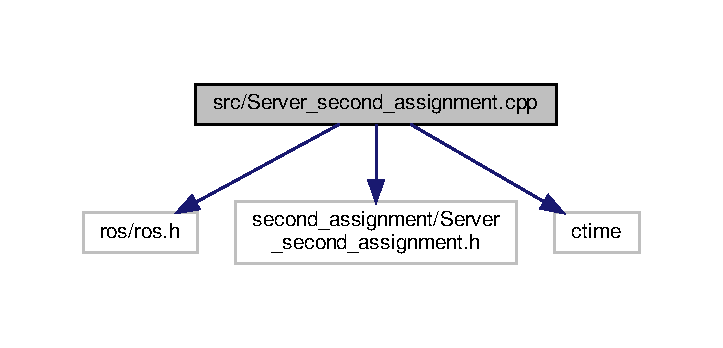
\includegraphics[width=347pt]{_server__second__assignment_8cpp__incl}
\end{center}
\end{figure}
\subsection*{Functions}
\begin{DoxyCompactItemize}
\item 
bool \hyperlink{_server__second__assignment_8cpp_ab257242eb5cfc7d5ec26c79a644a099d}{myrandom} (second\+\_\+assignment\+::\+Server\+\_\+second\+\_\+assignment\+::\+Request \&req, second\+\_\+assignment\+::\+Server\+\_\+second\+\_\+assignment\+::\+Response \&res)
\item 
int \hyperlink{_server__second__assignment_8cpp_a3c04138a5bfe5d72780bb7e82a18e627}{main} (int argc, char $\ast$$\ast$argv)
\end{DoxyCompactItemize}


\subsection{Function Documentation}
\mbox{\Hypertarget{_server__second__assignment_8cpp_a3c04138a5bfe5d72780bb7e82a18e627}\label{_server__second__assignment_8cpp_a3c04138a5bfe5d72780bb7e82a18e627}} 
\index{Server\+\_\+second\+\_\+assignment.\+cpp@{Server\+\_\+second\+\_\+assignment.\+cpp}!main@{main}}
\index{main@{main}!Server\+\_\+second\+\_\+assignment.\+cpp@{Server\+\_\+second\+\_\+assignment.\+cpp}}
\subsubsection{\texorpdfstring{main()}{main()}}
{\footnotesize\ttfamily int main (\begin{DoxyParamCaption}\item[{int}]{argc,  }\item[{char $\ast$$\ast$}]{argv }\end{DoxyParamCaption})}



Definition at line 25 of file Server\+\_\+second\+\_\+assignment.\+cpp.

\mbox{\Hypertarget{_server__second__assignment_8cpp_ab257242eb5cfc7d5ec26c79a644a099d}\label{_server__second__assignment_8cpp_ab257242eb5cfc7d5ec26c79a644a099d}} 
\index{Server\+\_\+second\+\_\+assignment.\+cpp@{Server\+\_\+second\+\_\+assignment.\+cpp}!myrandom@{myrandom}}
\index{myrandom@{myrandom}!Server\+\_\+second\+\_\+assignment.\+cpp@{Server\+\_\+second\+\_\+assignment.\+cpp}}
\subsubsection{\texorpdfstring{myrandom()}{myrandom()}}
{\footnotesize\ttfamily bool myrandom (\begin{DoxyParamCaption}\item[{second\+\_\+assignment\+::\+Server\+\_\+second\+\_\+assignment\+::\+Request \&}]{req,  }\item[{second\+\_\+assignment\+::\+Server\+\_\+second\+\_\+assignment\+::\+Response \&}]{res }\end{DoxyParamCaption})}

Function to obtain a random position Generate a random number

Use the random number as an index for the array 

Definition at line 6 of file Server\+\_\+second\+\_\+assignment.\+cpp.


%--- End generated contents ---

% Index
\backmatter
\newpage
\phantomsection
\clearemptydoublepage
\addcontentsline{toc}{chapter}{Index}
\printindex

\end{document}
